%% IDE has R L T A 3
%% timetable has L R A 3 - pretty much the order of the 2009 examples.tex
% TODO for future: check taht loop demos, etc, use ":" rather than ","
% for string concatenation

\documentclass[12pt,a4paper,twoside]{article}
\usepackage{graphicx,fancyhdr}


\setlength{\parindent}{0cm}
\setlength{\parskip}{2ex plus1ex minus 0.5ex}

\addtolength{\evensidemargin}{-2.5cm}
\addtolength{\oddsidemargin}{-0.5cm}
\addtolength{\textwidth}{3cm}

\addtolength{\headheight}{0.2cm}
\addtolength{\topmargin}{-2.5cm}
\addtolength{\textheight}{2.5cm}

% \newcommand{\source}[1]{\textbf{\verb^#1^}}}
\renewcommand{\_}{\texttt{\symbol{95}}}
\addtolength{\fboxsep}{0.1cm}
\newcommand{\param}[1]{\textit{\textrm{\textmd{#1}}}}
\newcommand{\codebar}{\rule{\textwidth}{0.3mm}}
\newcommand{\todo}{\textbf{TODO}}

\newlength{\codelen}
\newcommand{\code}[1]
{\begin{center}\fbox{\parbox{16cm}{\texttt{#1}}}\end{center}}

\newcommand{\mission}[1]{\item[#1:]}
% \newcommand{\mission}[1]{\texttt{#1}\hspace{3mm}}

\fancyhead{}
\fancyhead[RO,LE]{\thepage}
\fancyhead[LO,RE]{Tealight User Manual}
\fancyfoot{}
\pagestyle{fancy}
% \pagestyle{empty}

\setcounter{secnumdepth}{1}

\newenvironment{bulletlist}
{
	\begin{itemize}
	\addtolength{\itemsep}{-1mm}
	% \setlength{\itemsep}{0ex}
	\setlength{\parsep}{0ex}
}
{
	\end{itemize}
}

\newenvironment{alphalist}
{
	\begin{enumerate}
	\setlength{\itemsep}{0ex}
	\setlength{\parsep}{0ex}
	\renewcommand{\labelenumi}{(\alph{enumi})}
}
{
	\end{enumerate}
}

\newenvironment{numericlist}
{
	\begin{enumerate}
	\addtolength{\itemsep}{-1mm}
	% \setlength{\itemsep}{0ex}
	\setlength{\parsep}{0ex}
}
{
	\end{enumerate}
}

\usepackage{hyperref}
\begin{document}

\centerline{\textbf{\LARGE Tealight User Manual}}
\vspace{0.5cm}
\centerline{August 2015}
\centerline{Author: Ian Davies}
\centerline{Based on ROBOC, by David Eyers (\texttt{David.Eyers@cl.cam.ac.uk})}
{ \parskip 1mm plus 1pt \tableofcontents }


\newpage
\section{ Usage}

In order to use Tealight, you will need a github account. Create one for free at \verb^http://github.com^.
When you have created your github account, navigate to \verb^http://tealight.github.io^ and click \verb^Login^.
You will be asked for your github credentials.

Once you have logged in, use the buttons on the home page or in the navigation bar to switch to one of
the tealight \textit{modes}. Modes will be explained in more detail below.

Here is the editor screen:

\begin{center}
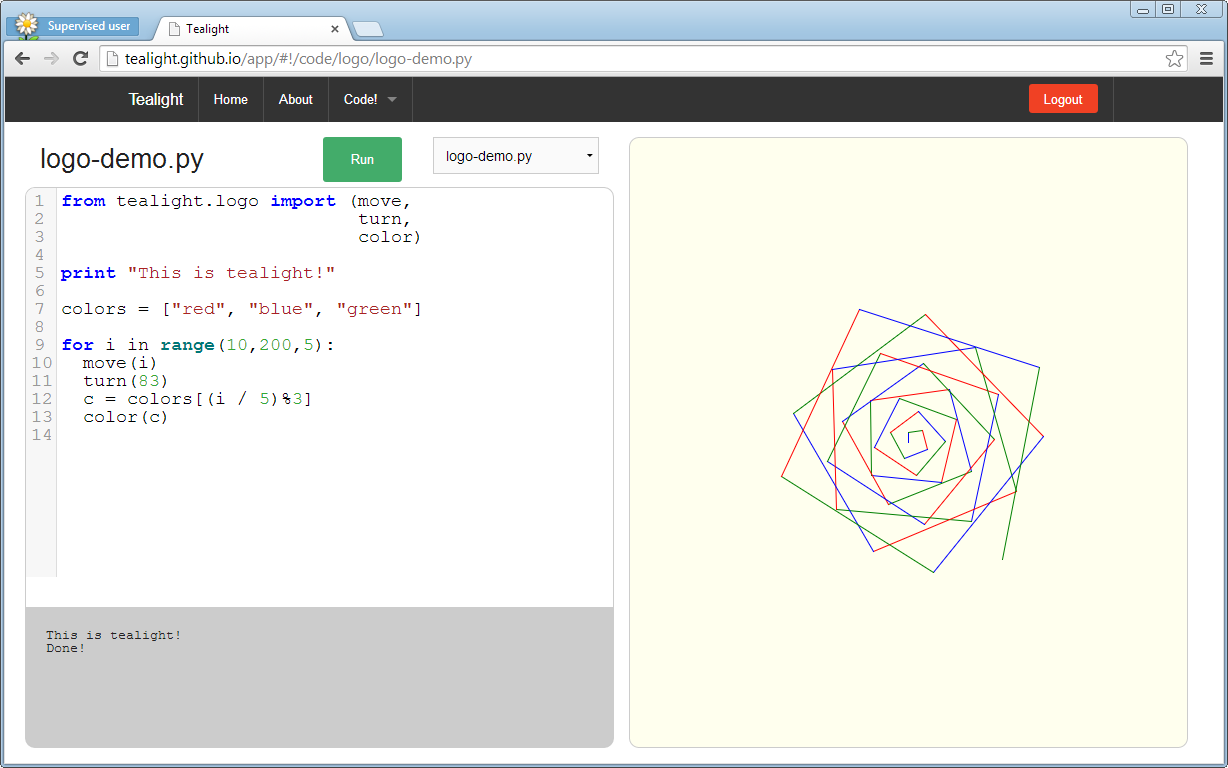
\includegraphics[scale=0.5,angle=0]{screenshots/ide/logo}
\end{center}

The drop-down box at the top allows you to switch between programs, or create new ones.
There are example programs in the box already that you can select from.

You should type your program into the main text area on the left. Any output text is displayed
on the gray console below, and the results of your program are shown on the right-hand panel.

\subsection{Running your program}

When you are ready to run your program, click the green \verb^Run^ button. When your program is running, you can \verb^Stop^ or \verb^Restart^ it. You can also use the keyboard shortcut \verb^Ctrl+Enter^ to run or restart your program.

Your program will be saved automatically every time you run it.

\subsection{Modes}

Tealight has three modes, usually introduced in order. To change mode, choose from the \verb^Code^ dropdown menu in the navigation bar. The modes are as follows:


\begin{tabular}{|l|l|}
\hline
Mode name & Manual page \\
\hline
Logo & \pageref{sec:logo-mode}\\
Robot & \pageref{sec:robot-mode}\\
Art & \pageref{sec:art-mode}\\ 
\hline
\end{tabular}

Most tealight features are available in all modes, but some are
mode-specific. Those are explained on their respective manual pages.

\subsection{Errors and Debugging}

It is \emph{very} easy to make mistakes when writing programs---most
people need a couple of tries before they get them right.
If there is a mistake in your program that prevents the computer
from understanding it, the program will stop. The line where the computer thinks
the mistake is will be highlighted in red, with a message describing the error. 
You should correct the mistake, then try running it again. Ask for help if you are still
stuck and can't see what the problem is.

\newpage
\section{The \textbf{\texttt{Python}} Language}

\subsection{Syntax}

\begin{bulletlist}
\item One statement per line
\item Blank lines and extra spaces are ignored by the interpreter
\item Blocks are denoted by indentation. The line that starts the block must
    end with a \verb^:^ and subsequent lines should be indented.
\item Python is case-sensitive. The word `python' is different to the word `Python'.
\end{bulletlist}

\subsection{Comments}

\begin{bulletlist}
\item Comments start with the \verb^#^ character and continue until the end
      of the line
\end{bulletlist}


\subsection{Names}

\begin{bulletlist}
\item Names are strings of letters, numbers and underscores
\item Names may not contain other characters, such as spaces or punctuation
\item Names must not start with a number
\item Capitalisation matters
\end{bulletlist}

\subsection{Keywords}

There are many keywords in Python. They are reserved, and cannot be used for anything else. They must be entered in lower case. Here are some of them:

{\bfseries \ttfamily
\begin{tabular}{|llllllllll|}
\hline
def & return & if & else & elif & for & while & continue & print & pass\\
\hline
\end{tabular}
}

Functions are defined with the \verb^def^ keyword. The program starts with the first command that is not a function
definition

\subsection{Variables}

\begin{bulletlist}
\item Variables consist of global variables, function parameters,
	loop counter variables and local variables
\item Loop counter variables are implicitly defined by the \verb^for^
	instruction, and function parameters by the function definition
\item Variables are declared implicitly by assignment to them
\item Assigning to a variable in a function creates a new local variable,
    even if a global variable exists with the same name.
\item To assign to a global variable inside a function, the variable must
    be declared \verb^global^ at the start of the function.
\item Any variable may hold either an integer, a number or some text, a list or an object.
\item Data types are not declared and all variables are named in the same way
\end{bulletlist}

Example:
\begin{verbatim}
speed = 0

def my_function(x,y):
    global speed
    speed = speed + x # This assigns to the global variable 'speed'

    z = x + y # This creates a new local variable 'z'

\end{verbatim}

\subsection{Text strings}

\begin{bulletlist}
\item String constants appear in ``double quotes'' or `single quotes'
\item Strings may be compared for equality or lexicographic ordering
	using the normal comparison statements
\item Strings may be joined with the \verb^+^ operator
\item Integers and other numbers are automatically converted to text
	when required
\item Strings can be converted to numbers with the \verb^int^ and \verb^float^ functions.
\end{bulletlist}

Example:
\begin{verbatim}
a = "foo"
b = "bar"
c = a + " " + b

d = "34" # This is a string, not a number!

e = int(d) # This is a now the number 34.
\end{verbatim}

\subsection{Expressions}

\begin{bulletlist}
\item The seven arithmetic operators are \verb^+ - * / % **^ (add,
	subtract, multiply, divide, remainder, exponentiate)
\item Division of integers will only return an integer. e.g. \verb^5 / 2 = 2^
\item To divide integers exactly, convert one to a float. e.g. \verb^5 / 2.0 = 2.5^
\item Remainder works with whole numbers, e.g. \verb^20 % 9 = 2^
\item The \verb^* /^ and \verb^%^ operators have higher precedence
                               (i.e.\ order of operations) than
	\verb^+^ and \verb^-^ (the first three kinds are evaluated first)

\item Operators of equal precedence are always evaluated left to right
\item Sub-expressions may be grouped with parentheses
\item Assignment is different from testing for equality. \verb^x = 3^ sets the value of \verb^x^ to \verb^3^, while \verb^x == 3^ returns \verb^True^ if \verb^x^ is equal to \verb^3^ and \verb^False^ otherwise.
\end{bulletlist}

Example:
\begin{verbatim}
speed = distance / stop - start
\end{verbatim}

\subsection{Libraries}
\label{subsec:libraries}
Some python functions, like \verb^len()^ and \verb^str()^ are built-in and available everywhere. Others need to be \textit{imported} explicitly. For instance, to use math functions you will need to import the \verb^math^ library:

\begin{verbatim}
import math

x = math.sin(2 * math.pi)
\end{verbatim}

Alternatively, you can import specific functions into the current file so that they can be called directly:

\begin{verbatim}
from math import sin, pi

x = sin(2 * pi)
\end{verbatim}

You will see this syntax later when we make use of the tealight libraries. For example:

\begin{verbatim}
from tealight.utils import sleep

sleep(500)
\end{verbatim}


\subsection{Conditional (\texttt{if}) statements}

\begin{bulletlist}
\item \verb^if^ statements are used to make decisions within a program
\item The four comparison operators are \verb^< > == !=^
\item \verb^!=^ means ``not equal''
\item The special values \verb^True^ and \verb^False^ are allowed
      instead of a comparison
\item Comparisons can be chained together with \verb^and^ and \verb^or^, and modified with \verb^not^.
\item There are optional \verb^else^ and \verb^elif^ blocks
\end{bulletlist}

Examples:
\begin{verbatim}
if lives == 0:
   end_game()


if item == Door and keys != 0:
   next_level()
elif monster_distance() < 2
   lives = lives - 1
end
\end{verbatim}

\subsection{Loops}

\begin{bulletlist}
\item Loops are a way to repeat the same set of actions
\item \verb^while^ loops repeat as long as the condition is true
\item \verb^for^ implicitly sets the value of a `counter' variable to each value in a list.
\end{bulletlist}

Examples:
\begin{verbatim}
n = 1
while n < 11:
   print n + " squared is " + (n * n)
   n = n + 1

while True:
   print "forever"

for n in range(0,10):
   print n + " squared is " + (n * n)
\end{verbatim}

\subsection{Functions}

\begin{bulletlist}
\item Functions blocks may be defined with the \verb^def^ keyword
\item Functions may be defined inside other functions
\item Functions may take any number of parameters
\item At run-time functions may call each other recursively
\item Parameters are separated by commas and listed in parentheses
\item Functions must be defined before they are called
\end{bulletlist}

Example:
\begin{verbatim}
from math import sqrt

def factorise(n):
   for i in range(2, int(sqrt(n))+1):
      if n % i == 0:
         print i
         factorise(n / i)
         return
   print n
        
factorise(100)
\end{verbatim}

\subsection{Lists}

\begin{bulletlist}
\item Lists are created with the \verb^list^ function or the literal \verb^[]^ syntax
\item List items are accessed with square brackets
\item Lists are indexed from zero.
\item Negative indices count backwards from the end of the list
\item Lists may be passed as arguments by reference (i.e.\ the one
  instance of the list will be shared between function caller and callee)
\item The \verb^len^ function returns the number of items in the list.
\end{bulletlist}

Example:
\begin{verbatim}
data = [1,1]

for i in range(0,10):
  data.append(data[-2] + data[-1])

print data
\end{verbatim}

\subsection{Dictionaries}

\begin{bulletlist}
\item Dictionaries map keys to values.
\item Dictionaries are created with the \verb^dict^ function or the literal \verb^{}^ syntax.
\item Dictionaries can be initialised, e.g. \verb^point = {`x': 10, `y': 20}^
\item To look up an item in a dictionary, use square brackets: \verb^point[`x']^
\item To delete an item from a dictionary, use the \verb^del^ keyword: \verb^del point[`x']^
\item Useful dictionary functions: \verb^clear, get, keys, values^
\end{bulletlist}

Example:
\begin{verbatim}
point = {`x': 10, `y': 20}

print point[`x']

point[`x'] = 12

del point[`y']
\end{verbatim}

\subsection{Output}

\begin{bulletlist}
\item \verb^print^ statements output text messages to the console.
\item You can print most types. They will be converted to strings and displayed.
\item There are many formatting functions available in python. Search online if required.
\end{bulletlist}

Example:
\begin{verbatim}
print "Score: " + points
print "Score: %d" % points
\end{verbatim}

\subsection{Standard math library} \label{sec:stand-math-libr}

These functions must be imported from the \verb^math^ library. For example, \verb^from math import sqrt^

\begin{verbatim}
y = sin(x)
y = cos(x)
y = tan(x)
y = sqrt(x)
y = pow(x, exponent)
y = log(x)
n = floor(x)
\end{verbatim}

The \verb^sin^, \verb^cos^ and \verb^tan^ functions all accept
arguments in radians. You can convert degrees to radians with the \verb^math.radians^ function, and radians to degrees with the \verb^math.degrees^ function.

You can also import the $\pi$ constant:

\begin{verbatim}
from math import pi
\end{verbatim}

\section{The \textbf{\texttt{Tealight}} Environment}

\subsection{Events}

Tealight programs can accept input through the \textit{event} system.

To handle events, you write special functions whose names begin with \verb^handle_^. For example, the following function will receive mouse move events:

\begin{verbatim}
def handle_mousemove(x,y):
  print `The mouse moved to ' + x + `,' + y
\end{verbatim}

Now, whenever the mouse moves over the main panel, your \verb^handle_mousemove^ function will be called.

When you define event handlers, your program does not stop executing when it reaches the end. It continues listening for events until you explicitly click the \verb^Stop^ button.

There are several built-in events raised by tealight. They are listed here, along with their optional arguments. When writing event handlers, you can choose to accept any of these arguments by name. Order is not important.

Built-in events:

\begin{bulletlist}
\item \verb^mousemove^

	Raised when the mouse moves over the right-hand panel where your program is executing. Provides arguments \verb^x^, \verb^y^ and \verb^button^, where \verb^x^ and \verb^y^ are in pixel coordinates ($y$ increases downwards, $(0,0)$ is in the top-left corner.) and \verb^button^ is one of \verb^None^, \verb^`left'^, \verb^`middle'^ and \verb^`right'^, indicating which mouse button is pressed, if any.

\item \verb^mousedown^

	Raised when a mouse button is pressed down. Provides the same arguments as \verb^mousemove^.
\item \verb^mouseup^

	Raised when a mouse button is released Provides the same arguments as \verb^mousemove^.
\item \verb^keydown^

	Raised when a key is pressed on the keyboard. Provides a single string argument, \verb^key^, which can be any lower-case letter (\verb^a^, \verb^b^, \verb^c^, etc.), any numeric character (\verb^0^, \verb^1^, \verb^2^, etc.) or any of the following values: \verb^up^, \verb^down^, \verb^left^, \verb^right^, \verb^backspace^, \verb^tab^, \verb^return^, \verb^escape^, \verb^delete^, \verb^space^, \verb^shift^, \verb^ctrl^, \verb^alt^.
\item \verb^keyup^

	Raised when a key is pressed on the keyboard. Provides the same arguments as \verb^keydown^.
\item \verb^frame^

	Raised approximately every ${1/60}^{th}$ of a second while your program is running. This is very useful if you wish to execute some graphics rendering in a loop while still receiving other events.
\end{bulletlist}

\subsection{Networking} \label{sec:networking-functions}

The tealight networking library allows your program to send and receive messages to and from other tealight programs running in other browsers, perhaps elsewhere in the world.

Start by importing the required functions:

\begin{verbatim}
from tealight.net import connect, send
\end{verbatim}

There are only two functions in the \verb^tealight.net^ library. They are used as follows:

\begin{bulletlist}
\item \verb^connect(app_name)^

	Connects to the tealight network server. You must do this before you can send or receive messages. Set \verb^app_name^ to something unique - when you send messages, they will be sent to every running program with the same \verb^app_name^. Similarly, you will receive messages from any program that set the same \verb^app_name^.

\item \verb^send(message, echo=False)^

	Sends a message to every tealight program connected with the same \verb^app_name^ as yours. \verb^message^ can be any simple type. Strings, numbers, lists and dictionaries are all supported. Setting the optional \verb^echo^ argument to \verb^True^ will cause the message to be sent back to your program in addition to being sent to remote receivers.
\end{bulletlist}

To receive messages, simple handle the \verb^message^ event, which takes one argument: \verb^message^.

\begin{verbatim}
def handle_message(message):
  print "Received message: " + message
\end{verbatim}

\subsection{Collaboration}

Tealight can be used for group-work as well as individual programming. You can include code from other users in your own program as follows:

\verb^import github.<username>.<mode>.<file>^

You should replace \verb^<username>^, \verb^<mode>^ and \verb^<file>^ as appropriate. For example:

\verb^import github.daviesian.art.my_file^

Notice that you do not include the \verb^.py^ extension at the end of the file name here.

As with normal imports (described on page \pageref{subsec:libraries}), you can also import specific functions from other users' files:

\verb^from github.daviesian.art.my_file import my_func, my_other_func^

If a user's Github username is not a valid Python identifier (e.g. contains hyphens), see the \verb^github_load^ function below.

\subsection{Other utilities}

The \verb^tealight.utils^ library contains functions that may be of general use when writing tealight programs:

\begin{bulletlist}
\item \verb^sleep(milliseconds)^

	Pauses execution of your program for \verb^milliseconds^ ms. Use this function with care -- you will be unable to receive events while your program is sleeping. You should use the \verb^frame^ event for animations, etc.

\item \verb^now()^

	Returns the current time, as a number of seconds since midnight on 1$^{st}$ Jan, 1970.

\item \verb^age()^

	Returns the length of time, in seconds, since your program started running.
\item \verb^github_load(username, mode, file)^

	Loads a remote file into the current file, returning a module object. Useful when the owner of the remote file has a Github username that is not a valid Python identifier.

\end{bulletlist}


\newpage
\section{Logo Mode} \label{sec:logo-mode}

In logo mode your Tealight program controls a turtle that paints
a line as it moves around on the screen. The turtle itself is
not shown and the output screen is initially blank.

You must import the \verb^tealight.logo^ functions in order to use them:

\begin{verbatim}
from tealight.logo import move, turn, color
\end{verbatim}

\subsection{Turtle control}

\begin{bulletlist}
\item \verb^turn^ and \verb^move^ control the turtle
\item Angles are measured clockwise in degrees
\end{bulletlist}

For example:
\begin{verbatim}
from tealight.logo import move, turn, color

turn(45)
move(100)
turn(-90)
\end{verbatim}

\subsection{Other functions}

\begin{bulletlist}
\item The \verb^color^ function changes the color of the line drawn by the turtle:

	\begin{verbatim}
	color("red")
	move(20)

	color("#0f0")
	move(20)

	color("rgba(0,0,255,0.5)")
	move(20)
	\end{verbatim}
\end{bulletlist}



\newpage
\section{Robot Mode} \label{sec:robot-mode}

In robot mode the aim is to steer a small robot around different
environments, navigating around walls and collecting fruit. The
fruit looks different on each map (diamonds, footprints, fuel canisters and so on), but
walls are always gray.

\begin{center}
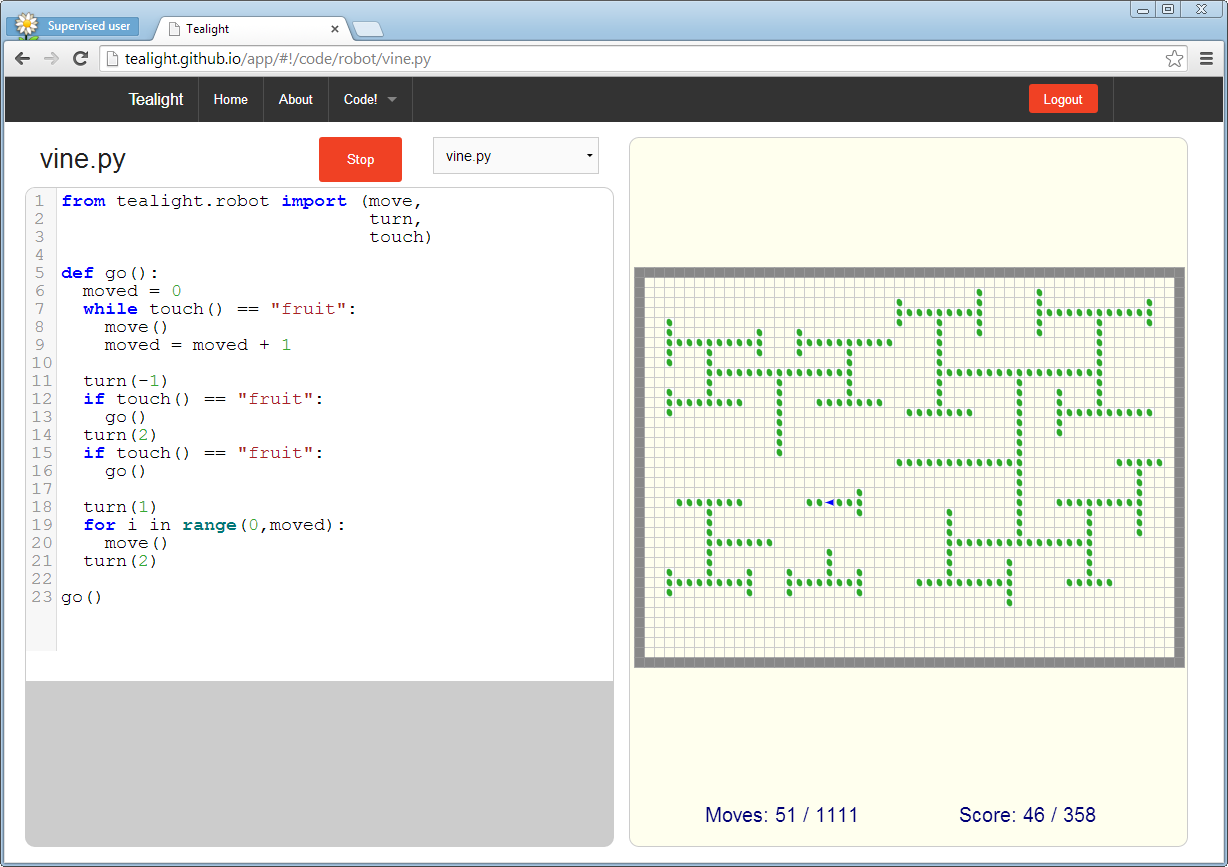
\includegraphics[scale=0.5,angle=0]{screenshots/ide/robot}
\end{center}

You must import the \verb^tealight.robot^ functions in order to use them:

\begin{verbatim}
from tealight.robot import move, turn, look, touch, smell, left_side, right_side
\end{verbatim}

\subsection{Movement}

In robot mode, you use the \verb^move^ and \verb^turn^
functions to control the robot. Note that, unlike logo mode, the robot turns in steps of 90 degrees clockwise and moves only one square at a time. The \verb^move^ function takes no parameters, and negative turns are anticlockwise. Here are some examples:

\begin{verbatim}
turn(-1)
move()
turn(1)
move()
turn(2)
\end{verbatim}


Here is a loop for moving more than one square
in a straight line:

\begin{verbatim}
distance = 10
for n in range(0, distance):
   move()

\end{verbatim}

\subsection{Senses}

There are five functions you can use to sense objects in the proximity
of the robot:

\begin{verbatim}
thing = touch()
thing = left_side()
thing = right_side()
thing = look()
count = smell()
\end{verbatim}

\begin{bulletlist}
\item \texttt{thing} will be one of:
	\texttt{None}, \texttt{`wall'} or \texttt{`fruit'}

\item \texttt{touch()} examines the square directly in front of the
	robot, \texttt{left\_side()} looks at the square immediately to its
	left and \texttt{right\_side()} looks at the square to its right.

\item \texttt{look()} looks forward in a straight line to the first
	non-empty square, however distant that might be.

\item \texttt{smell()} counts how many fruit are present
	in the 5x5 square portion of the grid centred on the robot.
\end{bulletlist}

Examples:

\verb^if touch() == `wall':^\\
\verb^   ^\textit{Do something}\\

\verb^if left_side() == `fruit':^\\
\verb^   ^\textit{Do something}\\

\verb^if right_side() != `wall':^\\
\verb^   ^\textit{Do something}\\

\verb^if look() == `fruit':^\\
\verb^   ^\textit{Do something}\\

\verb^if smell() > 2:^\\
\verb^   ^\textit{Do something}\\

\subsection{Usage instructions}

\textbf{Controls:}
Hold down the \textbf{ctrl} key to speed up the robot.

\textbf{Moves:}
The robot has a move limit set by the mission (for example, 400).
This is the number of time steps in which it must collect as much fruit
as possible. Any move or turn command takes one time step.

Calculations take no time..

\textbf{Scoring:}
Your robot scores 1 point per piece of fruit collected. 

\textbf{Target score:}
Every mission has a target score. You should try to reach this.
The target score isn't the highest possible on most missions, but
if you get it you know you have reached a good standard.

\newpage
\section{Art Mode} \label{sec:art-mode}

Art mode provides a blank canvas on which the program can draw.

You must import the \verb^tealight.art^ functions in order to use them:

\begin{verbatim}
from tealight.art import (line, 
                          spot, 
                          circle, 
                          box, 
                          rectangle, 
                          image, 
                          text, 
                          background, 
                          color)
\end{verbatim}

\subsection{Functions}

The coordinate system origin is at the top left corner of the
screen (graphics coordinates, with $y$ increasing downwards).

\begin{bulletlist}
\item \verb^line(x1, y1, x2, y2)^

	Draws a line from $(x_1,y_1)$ to $(x_2,y_2)$

\item \verb^line_width(width)^

	Sets the thickness of subsequently drawn lines.

\item \verb^circle(x, y, radius)^

	Draws a circle at $(x,y)$ with the specified radius

\item \verb^spot(x, y, radius)^

	Draws a filled circle at $(x,y)$ with the specified radius

\item \verb^rectangle(x, y, width, height)^

	Draws a rectangle with top-left corner at $(x,y)$ and with the specified width and height

\item \verb^box(x, y, width, height)^

	Draws a filled rectangle with top-left corner at $(x,y)$ and with the specified width and height

\item \verb^polygon(vertices)^

	Draws the outline of a polygon. The \verb^vertices^ argument should be a list of coordinate pairs, e.g. \verb^[(10,10), (20,10), (15,5)]^.

\item \verb^fill_polygon(vertices)^

	Draws a filled of a polygon. The \verb^vertices^ argument should be a list of coordinate pairs, e.g. \verb^[(10,10), (20,10), (15,5)]^.

\item \verb^test_polygon(x, y, vertices)^

	Returns \verb^True^ if the point $(x,y)$ lies inside the polygon defined by \verb^vertices^, otherwise returns \verb^False^. The \verb^vertices^ argument should be a list of coordinate pairs, e.g. \verb^[(10,10), (20,10), (15,5)]^.

\item \verb^image(x, y, file)^

	Draws one of the built-in images, listed on page \pageref{images}. The top-left corner is at $(x,y)$
\item \verb^text(x, y, string)^

	Draws the specified string at $(x,y)$. This is useful for writing any text to the screen.

\item \verb^font(f)^

	Sets the current font used by the \verb^text^ function. The argument \verb^f^ should be a string describing the font, e.g. \verb^"36px Verdana"^.

\item \verb^background(file)^

	Fills the screen with one of the built-in backgrounds, listed on page \pageref{backgrounds}
\item \verb^color(c)^

	Changes the current colour used by all the drawing functions. Use colour names (\verb^"red"^, \verb^"green"^, etc.), hexadecimal colours (\verb^"#ffea6d"^, \verb^"#FF0"^, etc.), RGBA colours (e.g. \verb^"rgba(255,128,0,0.5)"^) or HSL colours (e.g. \verb^"hsl(255,100%,50%)"^).
\end{bulletlist}

\subsection{Constants}

You can get the width and height of the screen in pixels. Import the constants as follows:
\begin{verbatim}
from tealight.art import screen_width, screen_height
\end{verbatim}


\subsection{Backgrounds}
\label{backgrounds}

The following backgrounds are available:
\begin{verbatim}
paper.jpg   track.png
\end{verbatim}

\newpage
\subsection{Images}

These are used with the \verb^image()^ function.

\label{images}
\small
\begin{tabular}{|l|l|l|l|}
\hline
\rule{0mm}{4.5mm}%
  animals/Ant.png         & food/Apple.png      & misc/Beachball.png       &  misc/Music.png\\
  animals/Bear.png        & food/Bananas.png    & misc/BlackBalloon.png    &  misc/OrangeBalloon.png\\
  animals/Butterfly.png   & food/Beer.png       & misc/BlueBalloon.png     &  misc/Paintbrush.png\\
  animals/Cat.png         & food/Burger.png     & misc/Boat.png            &  misc/Palette.png\\
  animals/Diplodocus.png  & food/Cake.png       & misc/Bomb.png            &  misc/PaperDart.png\\
  animals/Dog.png         & food/CandyCane.png  & misc/Boy.png             &  misc/Pencil.png\\
  animals/Dolphin.png     & food/Carrot.png     & misc/Card.png            &  misc/PinkBalloon.png\\
  animals/Dove.png        & food/Cheese.png     & misc/Clock.png           &  misc/PirateFlag.png\\
  animals/Elephant.png    & food/Cherries.png   & misc/Clover.png          &  misc/Pumpkin.png\\
  animals/Fish1.png       & food/Coffee.png     & misc/Cog.png             &  misc/RedBalloon.png\\
  animals/Fish2.png       & food/Croissant.png  & misc/Compass.png         &  misc/RedLight.png\\
  animals/Frog.png        & food/Fries.png      & misc/Daffodil.png        &  misc/Roller.png\\
  animals/Horse.png       & food/Glass.png      & misc/Dice.png            &  misc/Scissors.png\\
  animals/Ladybird.png    & food/Grapes.png     & misc/Drums.png           &  misc/Scroll.png\\
  animals/Lion.png        & food/IceCream.png   & misc/Flowers.png         &  misc/Snowman.png\\
  animals/Lobster.png     & food/Lemon.png      & misc/Football.png        &  misc/SuitClubs.png\\
  animals/Penguin.png     & food/Orange.png     & misc/Girl.png            &  misc/SuitDiamonds.png\\
  animals/Pterodactyl.png & food/Peach.png      & misc/GreenBalloon.png    &  misc/SuitHearts.png\\
  animals/Puffin.png      & food/Pie.png        & misc/GreenLight.png      & misc/SuitSpades.png\\
  animals/Seagull.png     & food/Pineapple.png  & misc/Harp.png            & misc/Sword.png\\
  animals/Seal.png        & food/Pizza.png      & misc/Heart.png           & misc/TeddyBear.png\\
  animals/Sheep.png       & food/Sandwich.png   & misc/HotAirBalloon.png   & misc/Tools.png\\
  animals/Siamese.png     & food/Strawberry.png & misc/Hourglass.png       & misc/Tulips.png\\
  animals/Stegosaurus.png & food/Tea.png        & misc/Lamp.png            & misc/Unlocked.png\\
  animals/Swan.png        & food/Watermelon.png & misc/Leaf.png            & misc/WhiteBalloon.png\\
  animals/Tiger.png       & food/Wine.png       & misc/Locked.png          & misc/WhiteFlower.png\\
                          &                     & misc/Luck.png            & misc/Wigwam.png\\
                          &                     & misc/MagicLamp.png       & misc/YellowBalloon.png\\
                          &                     & misc/MagnifyingGlass.png & misc/YellowFlower.png\\
                          &                     & misc/Mushroom.png        & misc/YellowLight.png\\
\hline
\end{tabular}
\normalsize

\end{document}
